
\section{\igh{} constant-region evolution in the Cyprinodontiformes}
\label{sec:comparative}

The characterised \igh{} loci of \nfu, \xma and medaka together reveal a high degree of variability in structure and function across the atherinomorph clade, with ... .


Many of these 

In this section, I address two of the most interesting of these questions, in particular the evolutionary history of 
	
In this section, I trace the evolutionary history of ...
	
In order to address these questions, I identified and analysed the \igh{} constant-regions present in a further ten cyprinodontiform species (\Cref{fig:species-tree-large-taxa}, \dots), % TODO: Table of analysed species and genomes
as well as a new and improved genome assembly of medaka (\dots), % TODO: Cite genome accession
using the same methods described for \Nfu and \Xma (\dots). % TODO: Cite methods description, describe manual refinement methods
Where possible, the indentified exons were then grouped by order and spatial proximity to identify contiguous constant-regions, enabling the presence/absence and number of constant regions of each isotype to be estimated for each species. % TODO: Table for this
Finally, the \cm{}, \cd{} and \cz{} exons so identified, along with those of \Nfu and \Xma identified in \Cref{sec:nfu-locus} and \Cref{sec:xma-locus}, were used to construct a large multiple-sequence alignment with \program{PRANK}, which was in turn used to build a phylogenetic tree of \ch{}-exon evolution in the Atherinomorpha.

 aligned with \program{PRANK}, and the resulting multiple-sequence alignment was used to build a phylogenetic tree of \ch-exon evolution 
 
 \begin{figure}
	\centering
	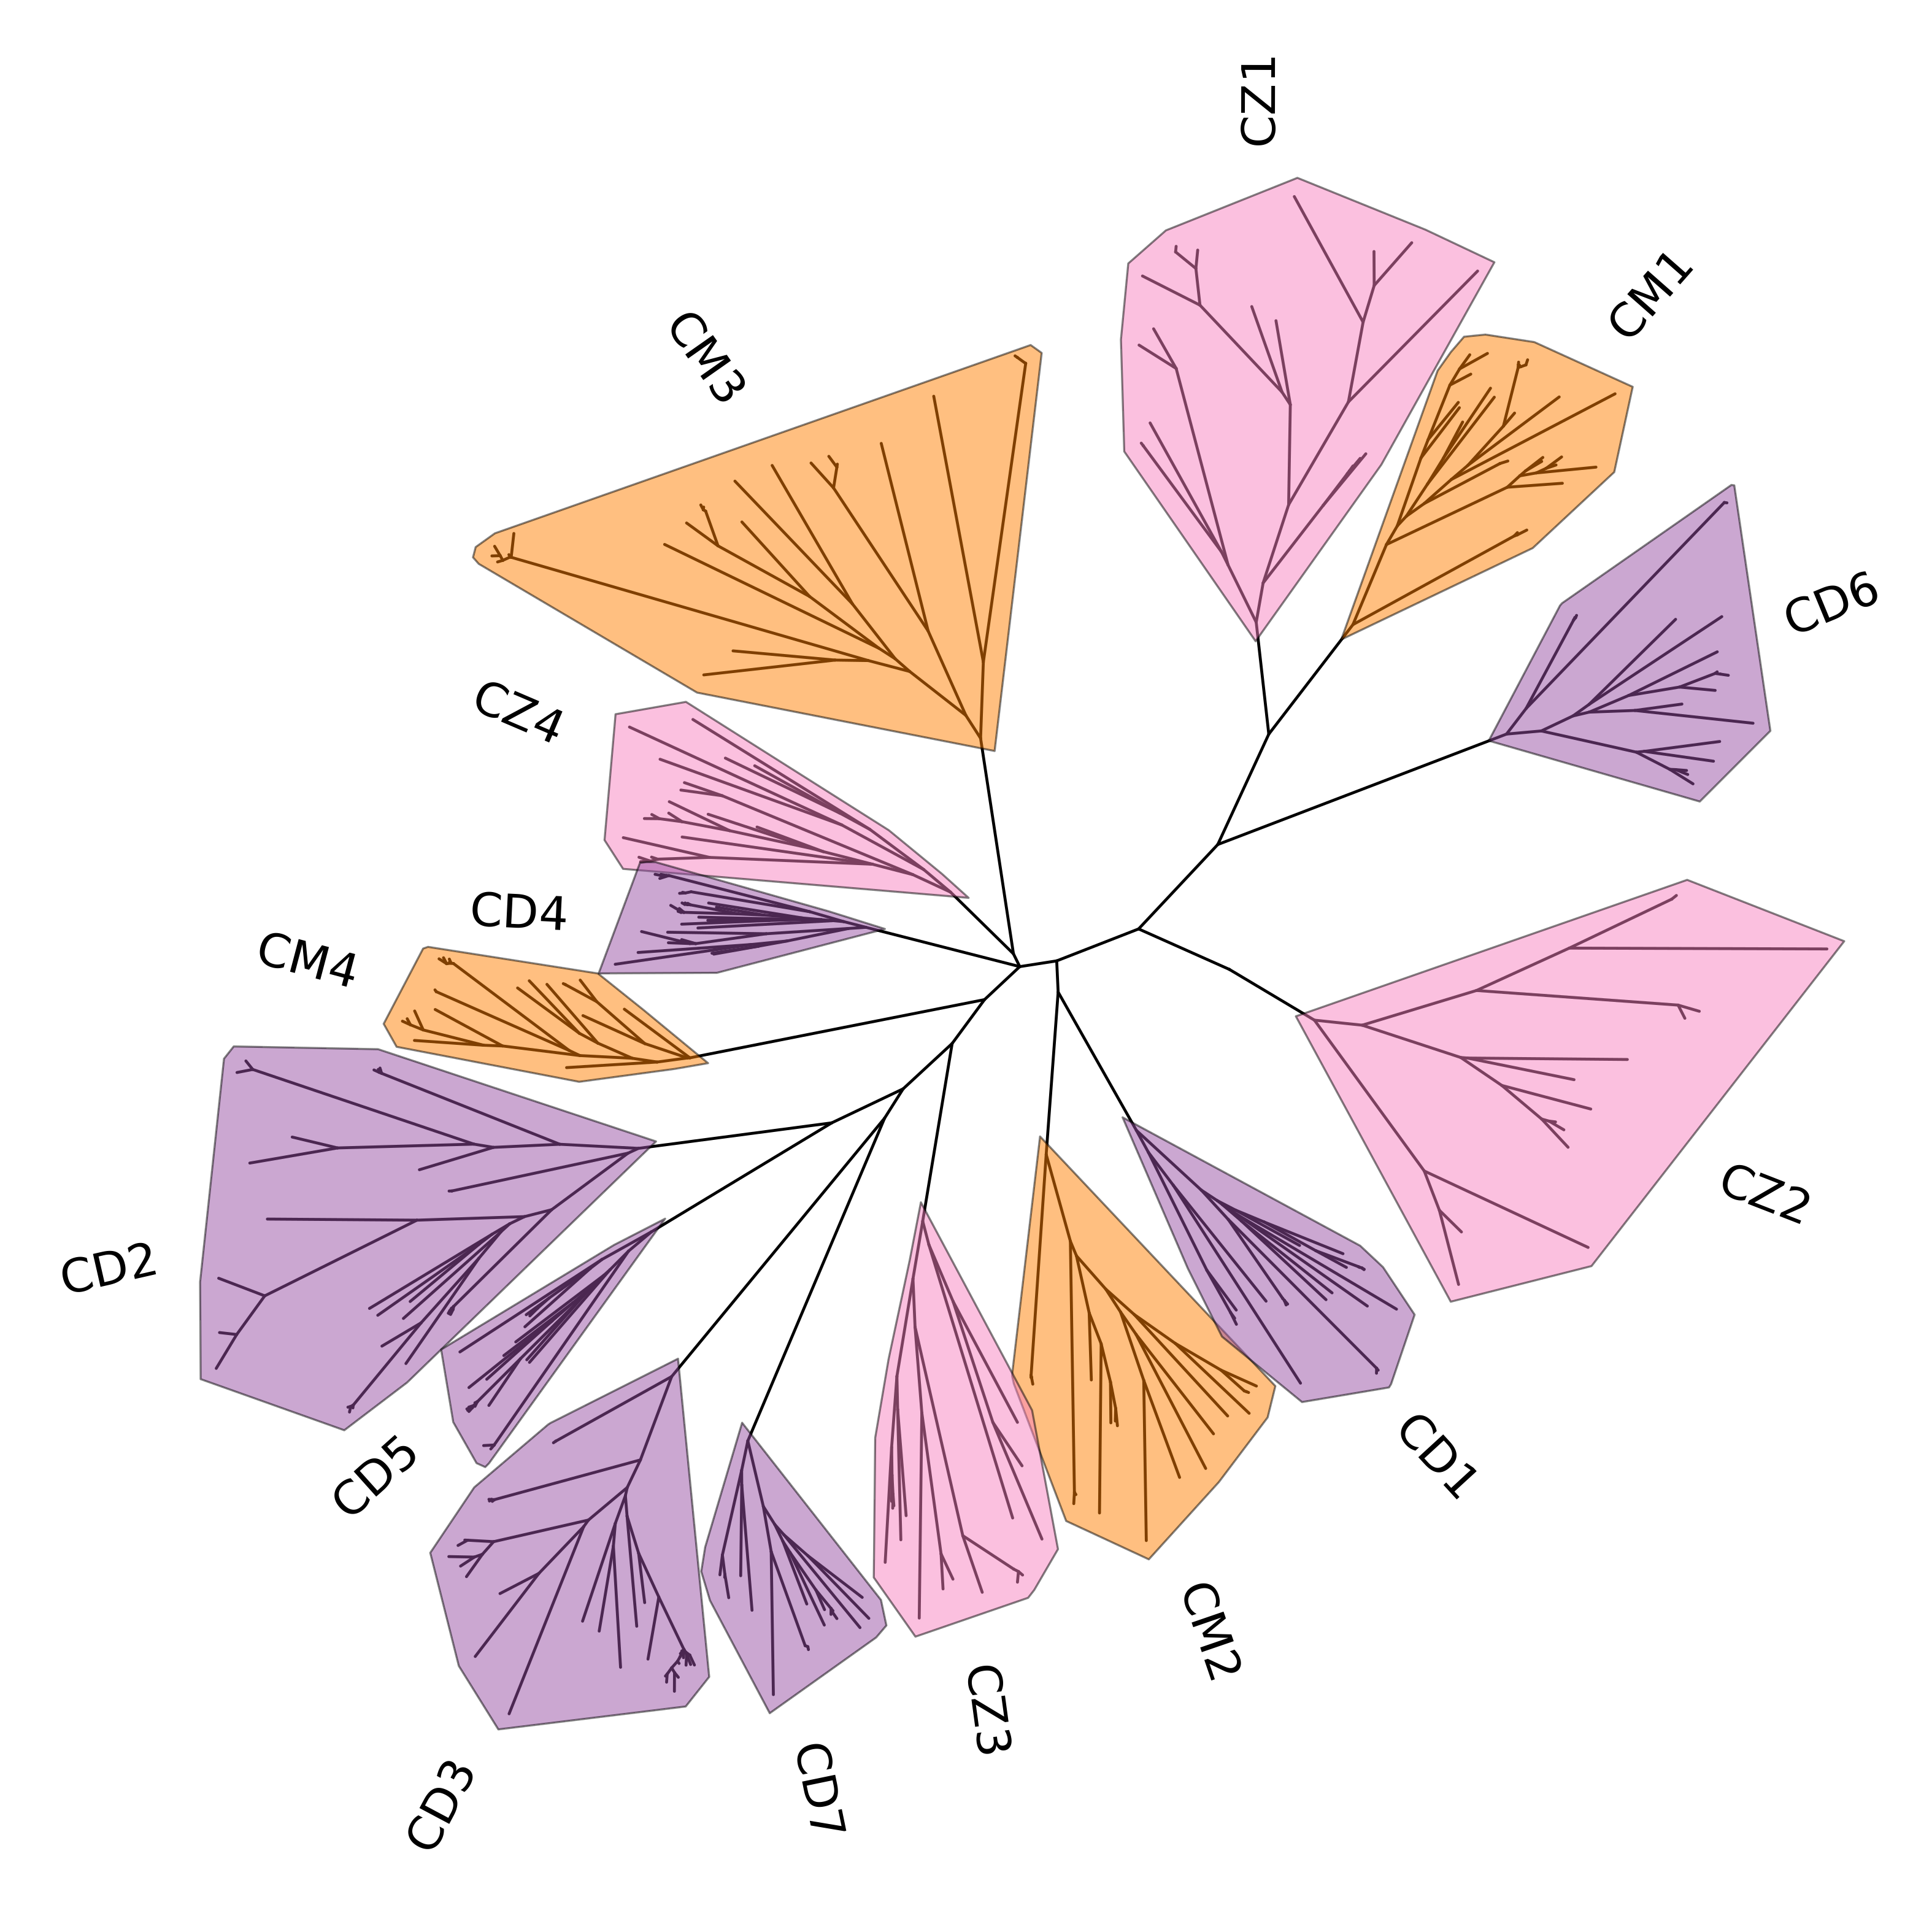
\includegraphics[width=0.9\textwidth]{_Figures/png/cyprinodontiform-ch-tree}
	\caption[\igh{Z} in the Atherinomorpha has been lost multiple times independently]{\textbf{\ch exons } Unrooted phylogram of \ch exons in \dots. %TODO: Denote species
	Each exon type is clustered separately in the tree topology and has been highlighted and labelled accordingly.}
	\label{fig:cyprinodontiform-ch-tree}
\end{figure} % TODO: Update tree


	\subsection{Evolutionary history of IgZ} % TODO: Better title
	
	The specialised mucosal isotype \igh{Z} is present in the majority of teleost \igh{} loci characterised so far, including several species (including stickleback and fugu) relatively closely related to the Atherinomorpha; the possession of \igh{Z} therefore appears to be primitive to most groups of teleost fish. The striking absence of the isotype in both medaka and turquoise killifish (\Cref{sec:nfu-locus-constant}), the first two characterised \igh{} loci from the Atherinomorpha, suggested that the lack of \igh{Z} may have occurred in the common ancestor of both species and so be primitive both the Beloniformes and Cyprinodontiformes; however, the surprising presence of two distinct \igh{Z} loci in the locus of the southern platyfish \xma convincingly falsified this hypothesis and indicated that the loss of \igh{Z} in medaka and turquoise killifish occurred independently in their respective lineages (\Cref{sec:xma-locus-constant}). 
	
	To further investigate the distribution and evolutionary history of \igh{Z} in the Cyprinodontiformes, \igh{Z} exons from zebrafish, stickleback and \Xma were aligned to the genomes of ten additional cyprinodontiform species (\dots) % TODO: Table of species
with \program{BLAST}, and the resulting alignments were processed as described in \dots % TODO: methods ref
to obtain complete exon sequences. This process revealed the presence of complete \igh{Z} constant regions (defined as \cz{1}-\cz{2}-\cz{3}-\cz{4}-TM1)% ; TM2 exons were not identified in most species due to the extreme shortness of their coding sequence) in 
in seven of the ten new species in addition to \Xma, including several species intermediate between \Xma and \Nfu (\Cref{fig:species-tree-large-ighz}) -- confirming that \igh{Z} is present in multiple cyprinodontiform species and that its absence in medaka and turquoise killifish most likely arose via multiple independent deletion events. Furthermore, only a single pseudogenised transmembrane exon (without accompanying \cz{} exons) could be found in the genome of \species{Austrofundulus limnaeus}, suggesting that functional \igh{Z} may also be absent in this species; if this is the case, it would represent a third independent loss event within the Atherinomorpha.

\begin{figure}
	\centering
	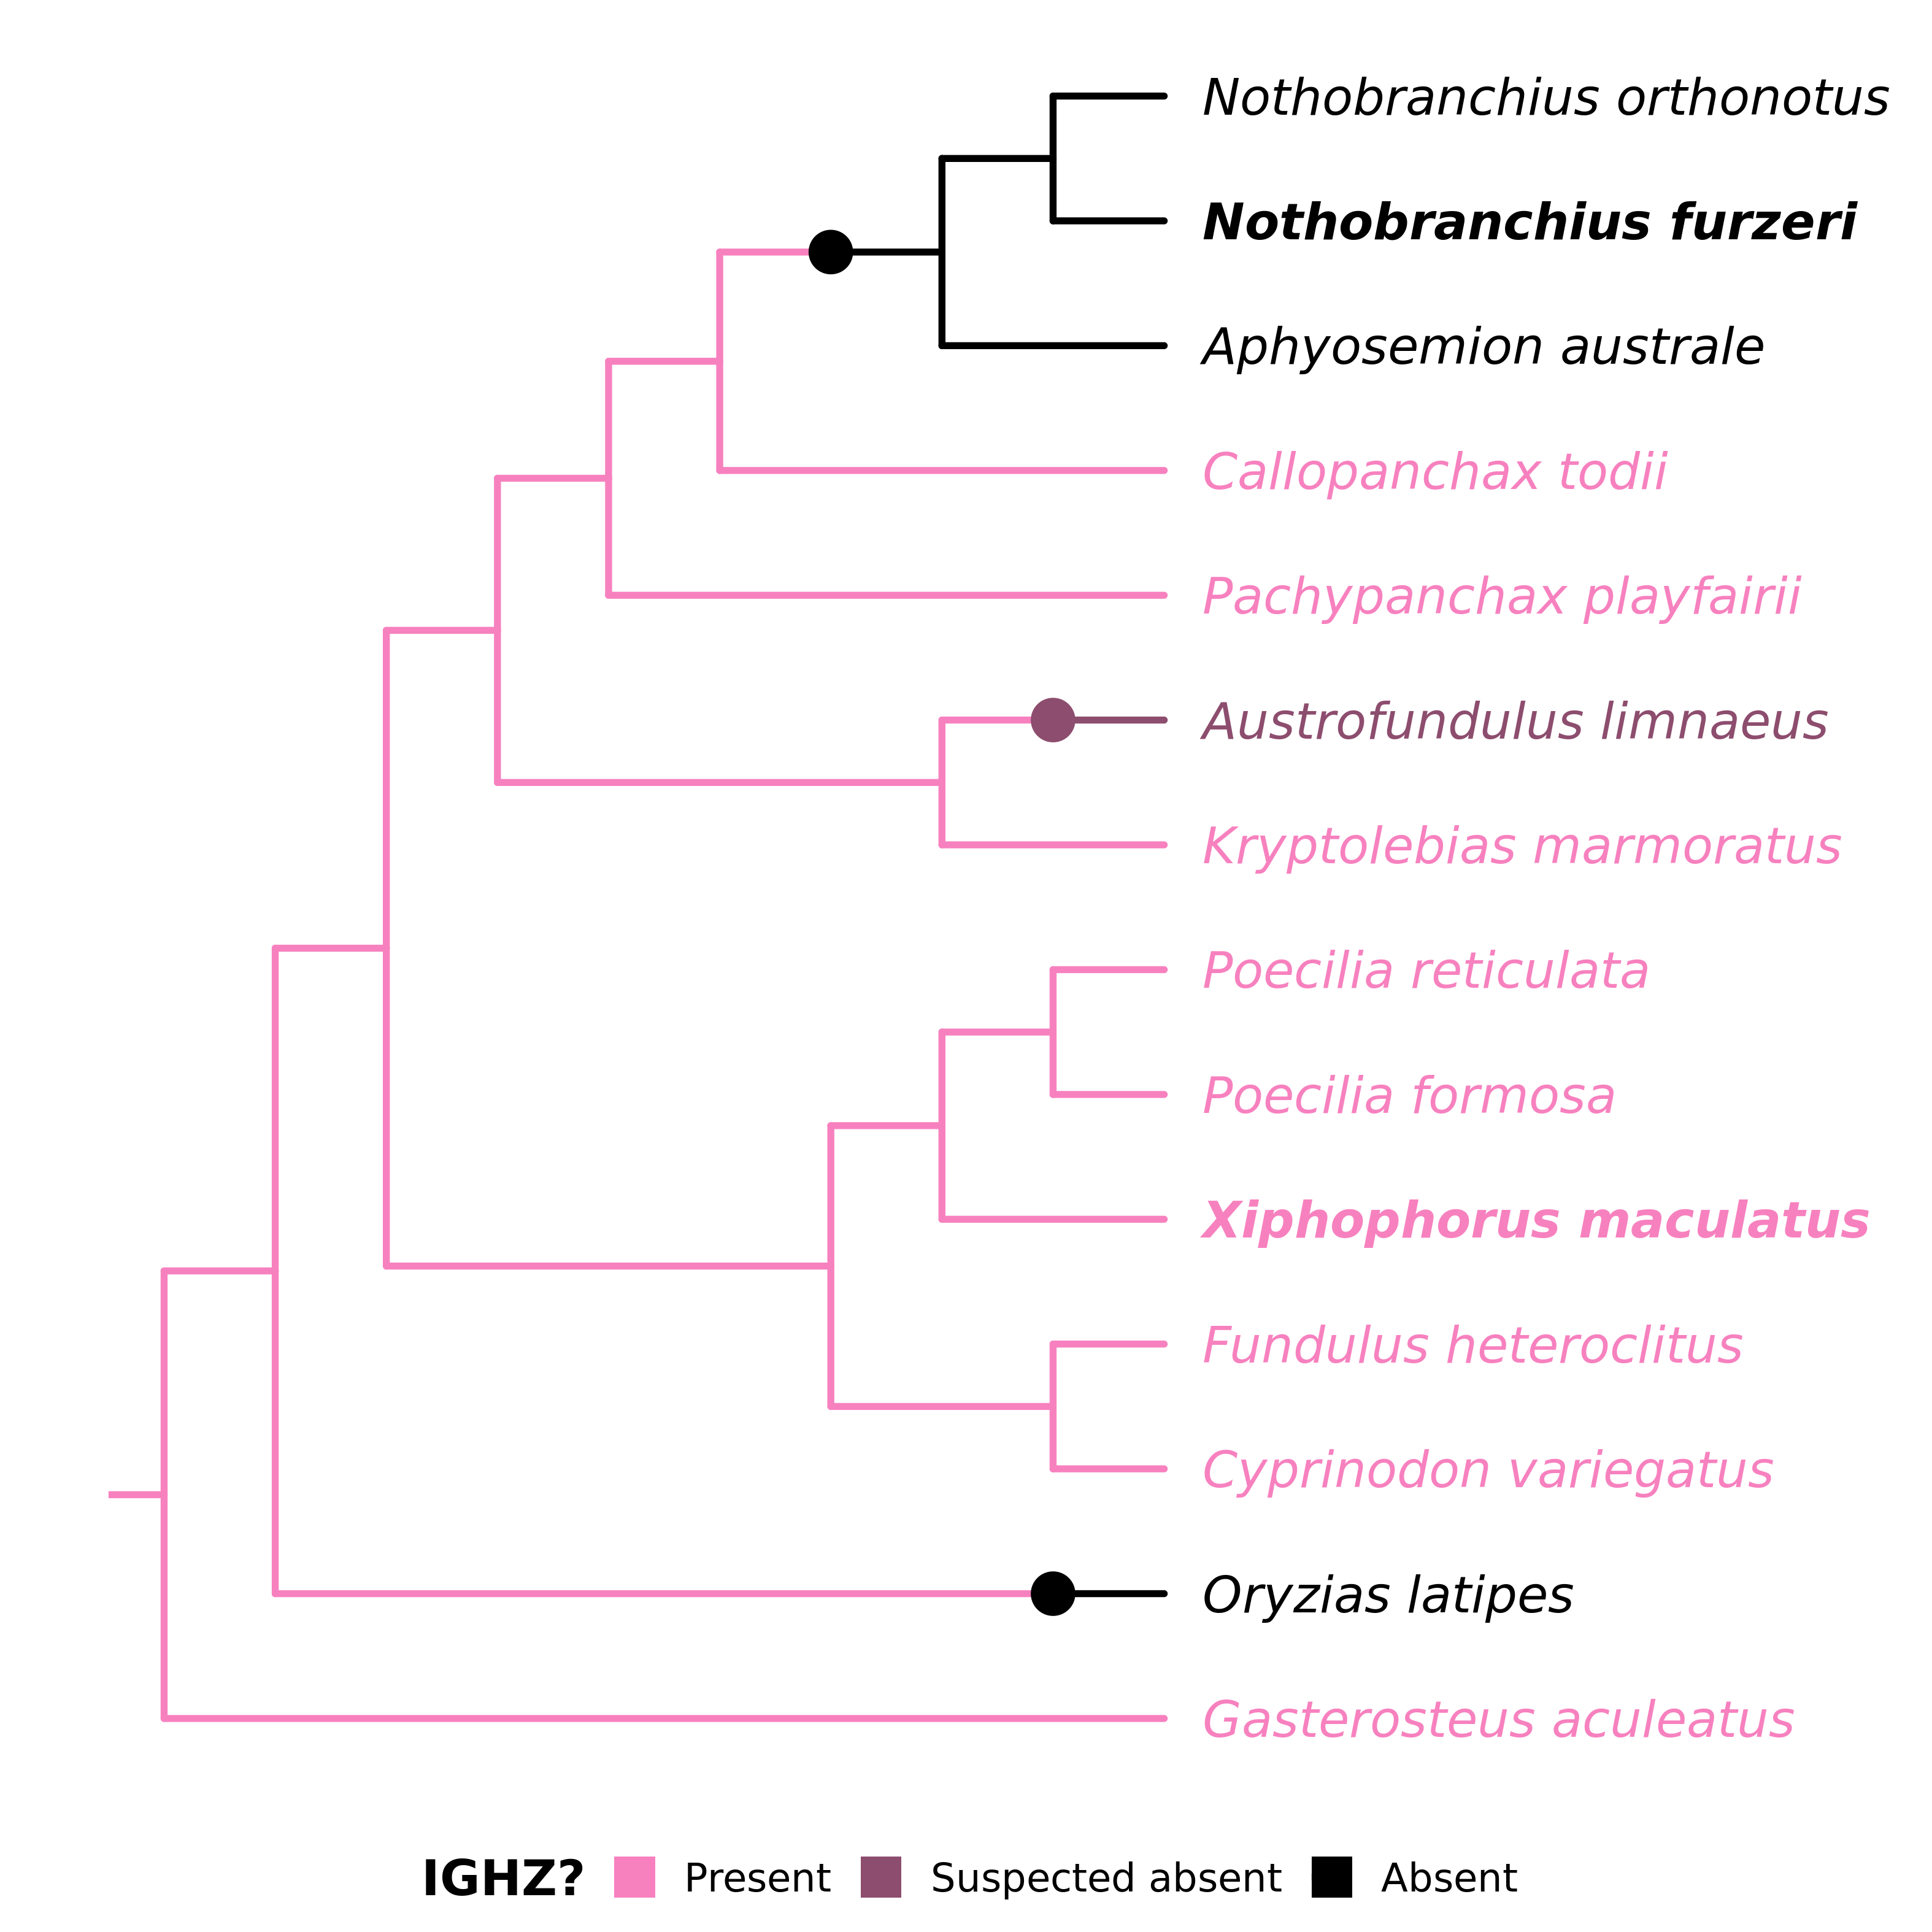
\includegraphics[width=0.9\textwidth]{_Figures/png/species-tree-large-ighz}
	\caption[\igh{Z} in the Atherinomorpha has been lost multiple times independently]{\textbf{\igh{Z} in the Atherinomorpha has been lost multiple times independently:} Cladogram of species reproduced from \Cref{fig:species-tree-large-taxa}, annotated according to the known (tip nodes) or hypothesised (internal nodes) presence or absence of intact \igh{Z} constant regions in each species. Large coloured points on the cladogram denote sites of hypothesised state changes; \igh{Z} is assumed to be primitively present in the clade and losses to be irreversible. The currently-available genome assembly of \textit{A. limnaeus} (purple) contains one pseudogenised \igh{Z-TM1} exon and no \cz{} exons.}
	\label{fig:species-tree-large-ighz}
\end{figure}

The \Xma \igh{} locus contains two distinct \igh{Z} constant regions, with only limited mutual sequence identity. % TODO: Ref figure and/or table here
Several other analysed species, including \dots, % TODO: species here
also exhibited multiple distinct \igh{Z} constant regions, suggesting a more complex pattern of \igh{Z} duplication and deletion than can be captured by a simple presence/absence metric. In order to better investigate the evolutionary history of \igh{Z} constant regions in the Cyprinodontiformes, the \cz{1}--\cz{4} nucleotide sequences of each observed constant region were concatenated together, aligned with \program{PRANK} and used to construct a phylogenetic tree with \program{RAxML}. 

The resulting tree (\Cref{fig:multispecies-cz-tree}) reveals three distinct lineages of \igh{Z} constant regions within the Cyprinodontiformes, each of which is present in multiple different species. Two of these, lineage A and B, correspond to \Xma \ighz{1} and \ighz{2}, respectively, while a third lineage C is represented in a close relative of \Xma (\species{Poecilia formosa}, the Amazon molly) but not \Xma itself. 

\begin{figure}
	\centering
	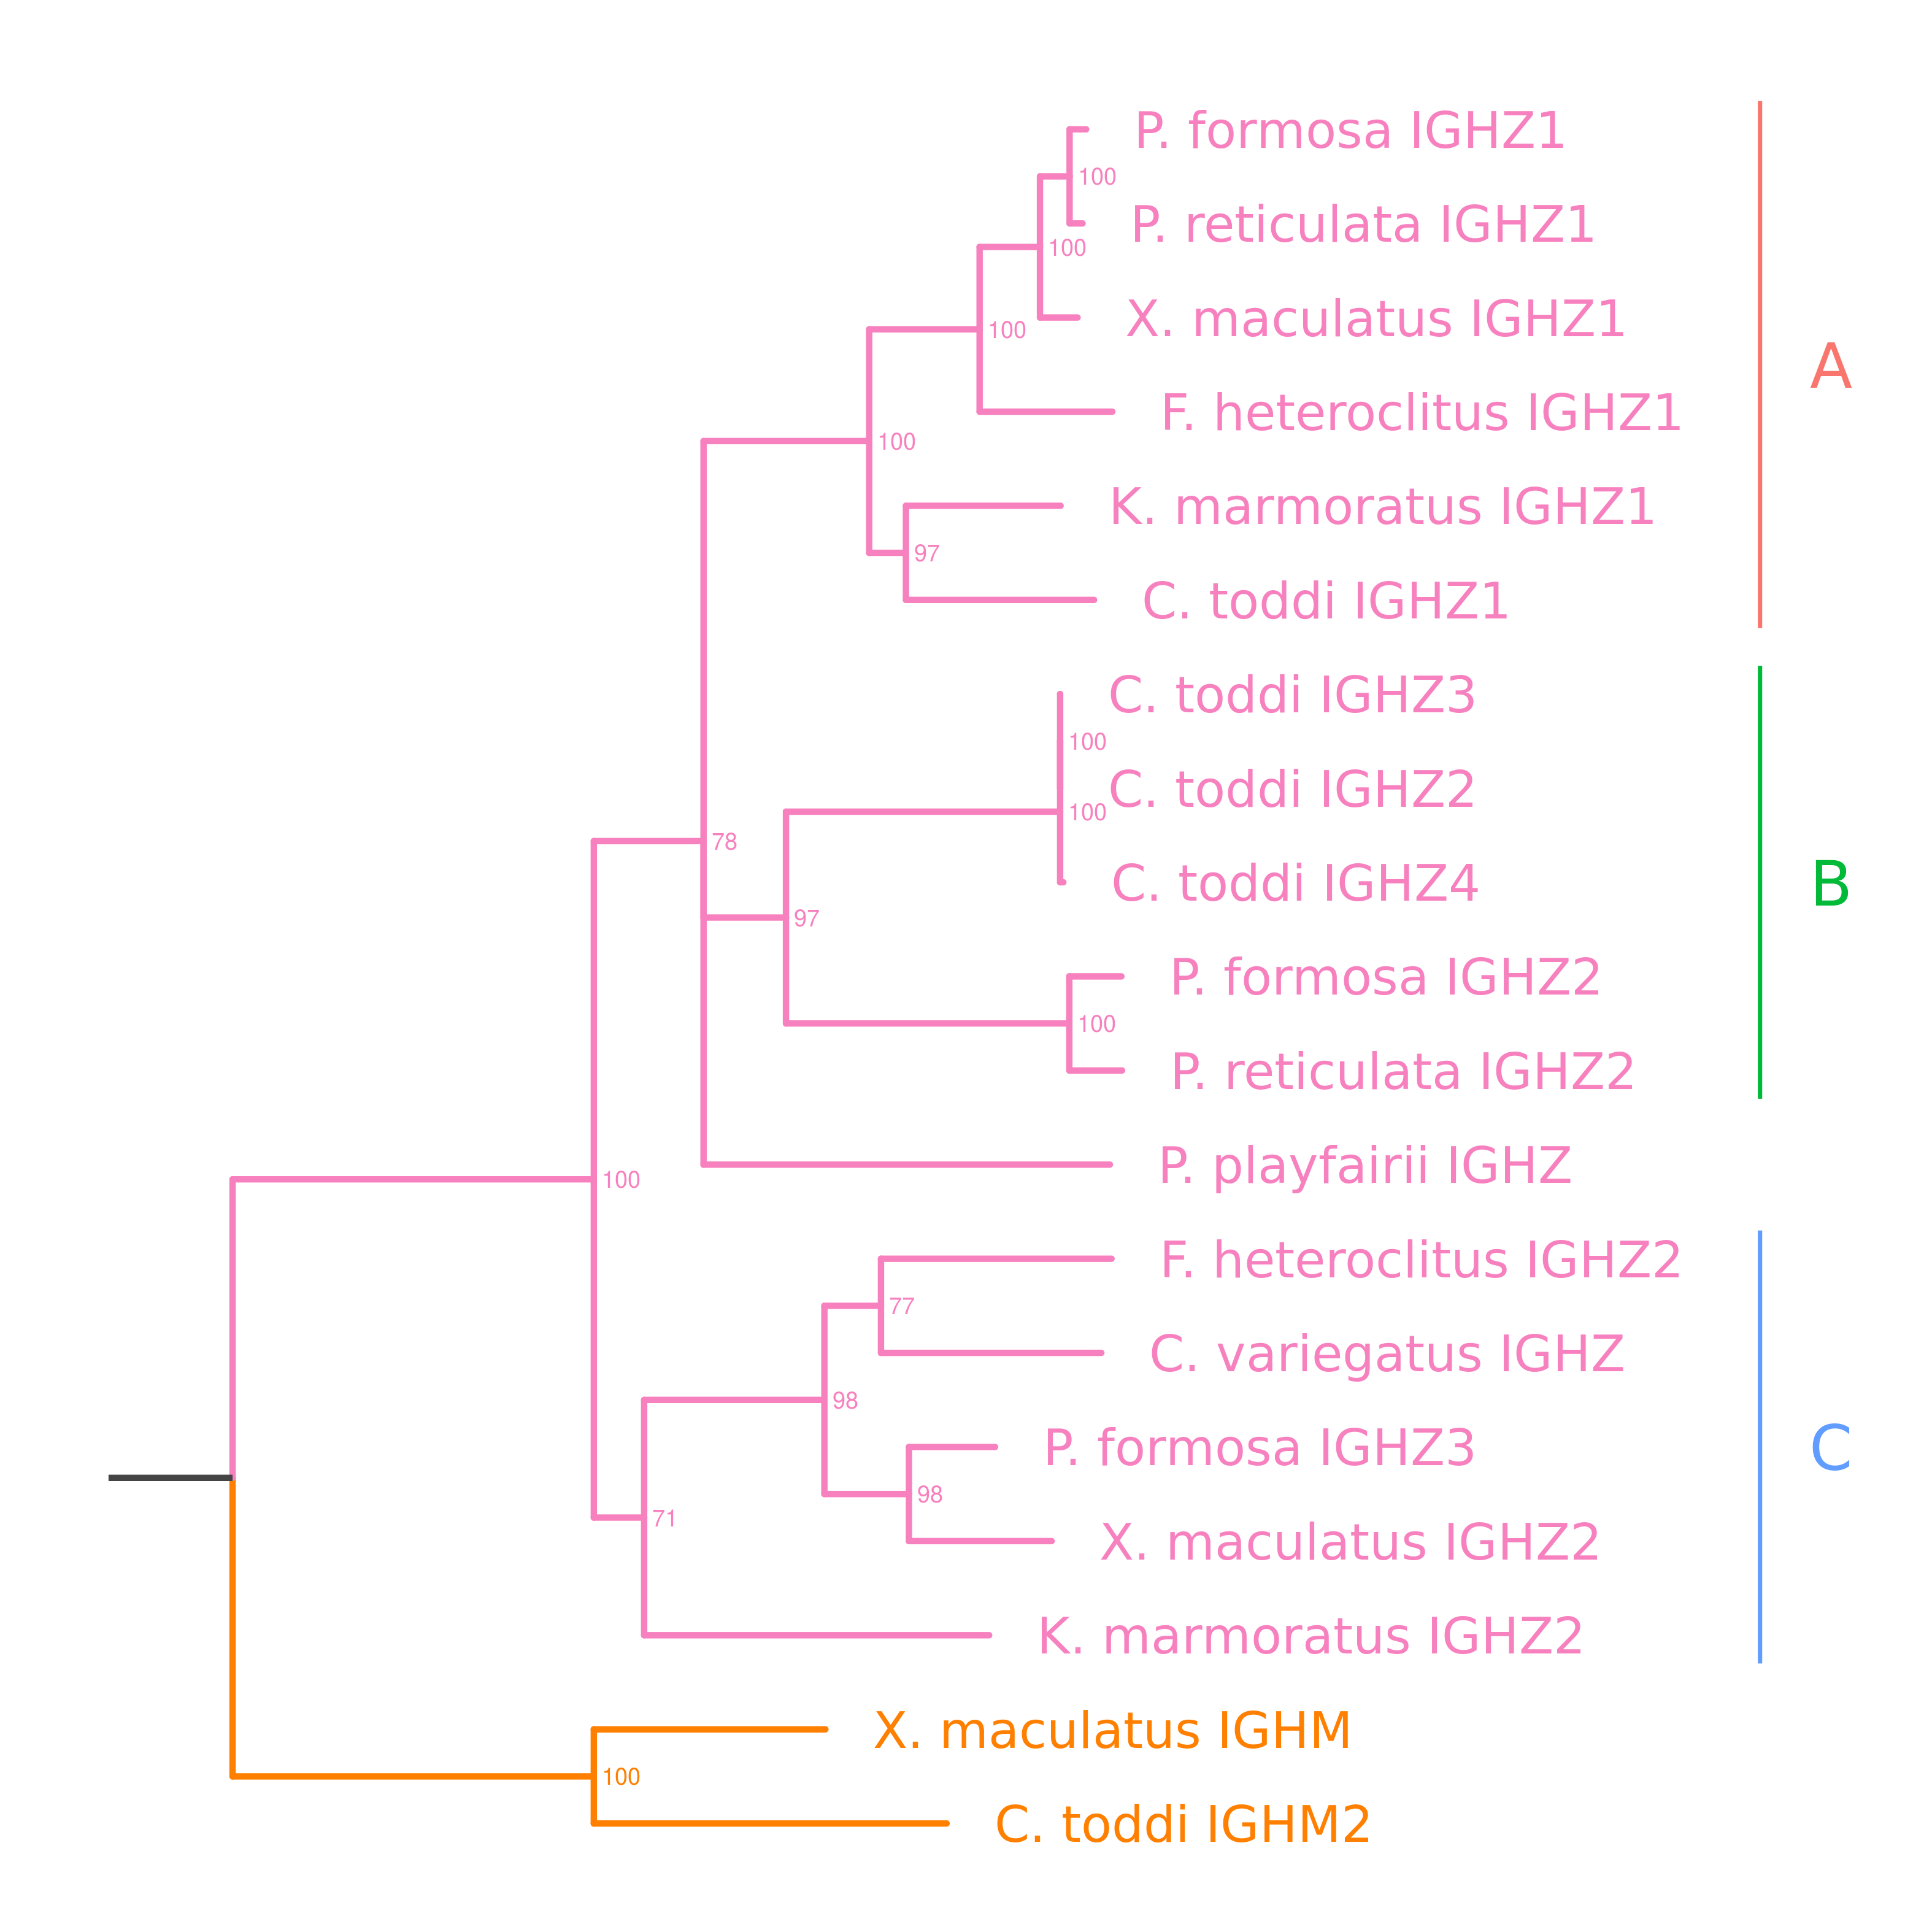
\includegraphics[width=0.9\textwidth]{_Figures/png/multispecies-cz-tree}
	\caption[\igh{Z} in the Atherinomorpha has been lost multiple times independently]{\textbf{\igh{Z} in the Atherinomorpha has been lost multiple times independently:} 
	Phylogram of concatenated \cz{1}--\cz{4} nucleotide sequences from \igh{Z}-bearing species from \dots % TODO: Designate species
	, with }
	\label{fig:multispecies-cz-tree}
\end{figure}

Only one \igh{Z} constant region from the analysed species could not be confidently assigned to one of these three lineages, namely the single \igh{Z} of \species{Pachypanchax playfairii}. In order to more closely investigate the relationships of \igh{Z} in this species, the exon sequences of \species{P. playfairii} \cz{1}--\cz{4} were separately aligned to the \cz{} exons of all other \igh{Z}-bearing species using Needleman-Wunsch global alignments, and the distribution of alignment scores was plotted in \dots % Figure
. The results show a striking difference in alignment behaviour between the exons, with \cz{1} and \cz{2} clearly aligning to exons from the B lineage and \cz{3} and \cz{4} showing more ambiguous affinity for either A- or C-lineage sequences. This unexpected behaviour suggests that the \species{P. playfairii} \igh{Z} sequence may be the result of a deletion or fusion event combining the first two exons of a B-lineage \igh{Z} constant region with the latter exons of a constant region from another lineage, resulting in a chimeric gene with ambiguous ancestry.

In summary, the cyprinodontiforms ancestrally possessed at least three variants of \igh{Z}, giving rise to multiple lineages of \igh{Z} constant regions evolving in parallel across the clade. Each of these lineages appears to have been lost in multiple cyprinodontiform species, with different species showing distinct patterns of retention and loss, and in at least one lineage -- that of \species{Pachypanchax playfairii} -- two different \igh{Z} lineages have fused to produce a chimeric isotype. All three lineages are missing from a subset of species in the Nothobranchiidae (including \nfu), and also appear to have been independently lost in \species{Austrofundulus limnaeus}. Taken together, these data suggest a high degree of complexity and volatility in the evolution of mucosal adaptive immunity in the Cyprinodontiformes.
	
	
	
	
	
	\subsection{Sublocus multiplicity and orientation}
	
	\subsection{Exon usage in transmembrane IgM \& other isoforms}


	%	The examination of the constant-region structures present in the \Xma IGH locus therefore reveals three notable features that differ in state between medaka, turquoise killifish, and the southern platyfish. Most strikingly, the absence of IGHM in medaka and killifish, but its presence in platyfish, strongly suggests that the isoform has been lost independently in the two groups. Conversely, the presence of a four-exon IGHM-TM in medaka and killifish, but a five-exon configuration in platyfish, is less clear-cut: it may indicate an independent change in medaka and killifish that is absent in platyfish, but may also plausibly represent a reversion in platyfish to the more-primitive five-exon state. Without a deeper understanding of the currently-unknown physical underpinnings of this observed difference in splicing behaviour, this question can only be addressed through analysis of RNA-seq data from a large number of related species, something beyond the scope of the present investigation. % TODO: Do it anyway?
%	Finally, the presence of a (\cd{2}-\cd{3}-\cd{4}) duplication in both platyfish and killifish, but not in medaka, suggests that this may be a shared primitive feature of the Cyprinodontiforms; however, given the apparent recurrence of this duplication pattern in many different groups across the teleosts, a strong conclusion cannot be drawn without a higher-resolution phylogenetic analysis of a larger number of related species. % TODO: See section ... etc.
% TODO: Move to multispecies section intro

	%	TODO: Move to multilocus section. Alongside this, I performed a more limited characterisation of the \textit{IgH} constant regions in 9 %?
%	additional cyprinodontiform and beloniform species, to assess the broader patterns of immunoglobulin heavy chain evolution within these groups (\Cref{sec:comparative-loci}). The results of these additional investigations repeatedly called into question the hypothesis of homology in IgH locus ideosyncracies between medaka and turquoise killifish, and suggest a model of rapid locus evolution within this diverse and important teleost clade.
	
	% TODO: Move to discussion section.
	% TODO: Relationship between killifish Vs and other species
	% TODO: Evolution of IGH1 vs 2
	% TODO: Discussion of mucosal immunity in absence of IGZ
		% TODO: Discuss smallness of killifish locus in the context of relaxed purifying selection and short life span
	% TODO: Section on "Investigating the evolutionary relationship between IGH1 and IGH2"
	% Keep for discussion:
%\q{Given the lack of IgZ in this species, how do you think they carry out mucosal immunity?}
%
%I'd assume using IgM. It's the primitive antibody and is expressed in secreted form in the killifish gut. I haven't investigated the protein expression so it's hard to say for sure, but I'd guess that's the answer. It's also quite possible, lacking a specialised mucosal class, that the answer is ``not very well". It would be very interesting to compare mucosal immune function in species with and without IgZ, especially if those species are closely related.
%
%Given the impressive results indicating the specificity of IgT for mucosal immunity in trout, and the lack of mucosal response of IgM in that species, it would be very interesting to see what mucosal responses look like in a species that lacks that isotype -- is IgM much more responsive and expressed in the gut than in IgT-possessing species, or is the mucosal response just worse?
	% (Incidentally, it would be great to see whether any B-cells in TK show recombinations in both subloci, vs one or the other. Single-cell DNA sequencing could plausibly do this.)








	



